\documentclass[12pt]{article}

\usepackage{bbm}
\usepackage{fancyhdr}
\usepackage{titling}
\usepackage{enumitem}
\usepackage{amsmath}
\usepackage{dsfont}
\usepackage{amsfonts}
\usepackage{amssymb}
\usepackage{amsthm}
\usepackage{geometry}
\usepackage{tikz}
\usepackage{algorithm}
\usepackage{algpseudocode}
\geometry{verbose,tmargin=1in,bmargin=1in,lmargin=1in,rmargin=1in}
\renewcommand{\vec}[1]{\mathbf{#1}}
\newcommand{\dec}{\text{dec}}
\newcommand{\divi}{\mathbin{\textnormal{div}}}
\title{Homework 1}
\author{Satvik Prasad}
\date{}
\newtheorem{lemma}{Lemma}[section]
\fancypagestyle{plain}{%
  \fancyhf{}
  \fancyhead[L]{\theauthor}
  \fancyhead[R]{\thedate}
}
\pagestyle{plain}
\makeatletter
\def\@maketitle{%
  \newpage
  \null
  \vskip 1em%
  \begin{center}%
    \let \footnote \thanks
    {\LARGE \@title \par}%
    \vskip 1em%
  \end{center}%
  \par
\vskip 1em}
\makeatother
\usepackage{cmbright}

\newcommand{\mat}[1]{\mathbf{#1}}

% ---------- Probability theory ----------
% Core operators (optional argument-free; use as \E{X}, \Var{X}, \Cov{X}{Y})
\DeclareMathOperator{\EOp}{\mathbb{E}}
\DeclareMathOperator{\VarOp}{Var}
\DeclareMathOperator{\CovOp}{Cov}
\DeclareMathOperator{\CorrOp}{Corr}

\renewcommand{\P}[1]{\mathbb{P}\left(#1\right)}        % \P{A}
\newcommand{\E}[1]{\EOp\left[#1\right]}                % \E{X}
\newcommand{\Var}[1]{\VarOp\left(#1\right)}            % \Var{X}
\newcommand{\Cov}[2]{\CovOp\left(#1,\,#2\right)}       % \Cov{X}{Y}
\newcommand{\Corr}[2]{\CorrOp\left(#1,\,#2\right)}     % \Corr{X}{Y}
\newcommand{\SD}[1]{\operatorname{SD}\left(#1\right)}  % \SD{X}

% Subscripted versions, e.g. \Esub{\theta}{X}, \Psub{\theta}{A}
\newcommand{\Esub}[2]{\EOp_{#1}\left[#2\right]}
\newcommand{\Psub}[2]{\mathbb{P}_{#1}\left(#2\right)}

% Conditioning, indicators, independence
\newcommand{\given}{\,\middle|\,}                      % \E{X \given Y}
\newcommand{\ind}[1]{\mathbbm{1}\left\{#1\right\}}     % \ind{X > 0}
\newcommand{\indep}{\perp\!\!\!\perp}                  % X \indep Y
\newcommand{\iid}{\overset{\text{iid}}{\sim}}          % X_i \iid \Normal(0,1)

% Convergence
\newcommand{\convp}{\xrightarrow{\;p\;}}               % in probability
\newcommand{\convd}{\xrightarrow{\;d\;}}               % in distribution
\newcommand{\convas}{\xrightarrow{\text{a.s.}}}        % almost surely
\newcommand{\convLp}[1]{\xrightarrow{L^{#1}}}          % in L^p

% Probability spaces
\newcommand{\F}{\mathcal{F}}                           % sigma-algebra
\newcommand{\B}{\mathcal{B}}                           % Borel sigma-algebra
\newcommand{\pspace}{(\Omega, \F, \mathbb{P})}

% Common distributions
\newcommand{\Normal}{\mathcal{N}}
\newcommand{\Bern}{\operatorname{Bernoulli}}
\newcommand{\Bin}{\operatorname{Binomial}}
\newcommand{\Pois}{\operatorname{Poisson}}
\newcommand{\Unif}{\operatorname{Uniform}}
\newcommand{\Exp}{\operatorname{Exp}}
\newcommand{\Geom}{\operatorname{Geometric}}
\newcommand{\Gam}{\operatorname{Gamma}}
\newcommand{\Beta}{\operatorname{Beta}}

% Number sets
\newcommand{\R}{\mathbb{R}}
\newcommand{\N}{\mathbb{N}}
\newcommand{\Z}{\mathbb{Z}}


\begin{document}
\begin{enumerate}
  \item
    \begin{enumerate}
      \item $\{\{a, b, c\}, \{d, e, g\}, \{f\}\}$

      \item $a, b, c, d, e, f, g$

      \item $f, e, g, d, c, b, a$
    \end{enumerate}

  \item We can track the predecessor node in the path from $s$ to $t$
    with something like the following:

    \begin{algorithm}
      \caption{DFS with path tracking}
      \begin{algorithmic}
        \Procedure{DFS}{$G$, $s$, $t$}
        \State $p = \{\}, \text{stk} = [s], \text{visited} \gets s$

        \vspace{3mm}

        \While{$\neg$empty(stk)}
        \State $c$ = stk.back()

        \vspace{3mm}

        \If{$c = t$}
        \State \textbf{break}
        \EndIf

        \vspace{3mm}

        \For{$n$ $\in G[c]$}
        \If{$n$ $\in $ visited}
        \State \textbf{continue}
        \EndIf
        \State visited $\gets$ $n$

        \vspace{3mm}

        \State $p[n] = c$
        \State stk.push($n$)
        \EndFor
        \EndWhile

        \vspace{3mm}

        \If{$t \not \in p$}
        \State \Return{\textbf{nil}} \Comment{No such path exists.}
        \EndIf

        \vspace{6mm}

        \State $c = t, $ path $= []$ \Comment{Determine path from predecessors.}
        \While{$c \neq s$}
        \State path.push\_front($c$)
        \State $c = p[c]$
        \EndWhile
        \State path.push\_front($s$)

        \vspace{3mm}

        \State \Return{path}
        \EndProcedure
      \end{algorithmic}
    \end{algorithm}

    \newpage

  \item Trees satisfy $|V| = |E| + 1,$ and must be completely
    connected. Hence, we must simply verify that $|V| = |E| + 1,$ in
    which case we can run a DFS in $\mathcal O(|V| + |E|) = \mathcal
    O(|V|)$ time to verify connectivity.

    \begin{algorithm}
      \caption{Graph is tree}
      \begin{algorithmic}
        \Procedure{IsTree}{$G$}
        \State $(V, E) = G$
        \If{$|V| \neq |E| + 1$}
        \State \Return{\text{false}}
        \EndIf

        \vspace{3mm}

        \State \text{visited} = DFS($G$)
        \For{$v \in V$}
        \If{$v \not \in \text{visited}$}
        \State \Return{false}
        \EndIf
        \EndFor

        \State \Return{true}
        \EndProcedure
      \end{algorithmic}
    \end{algorithm}

    \newpage
  \item
    \begin{enumerate}
      \item Edges are visited in this order:
        \begin{center}
          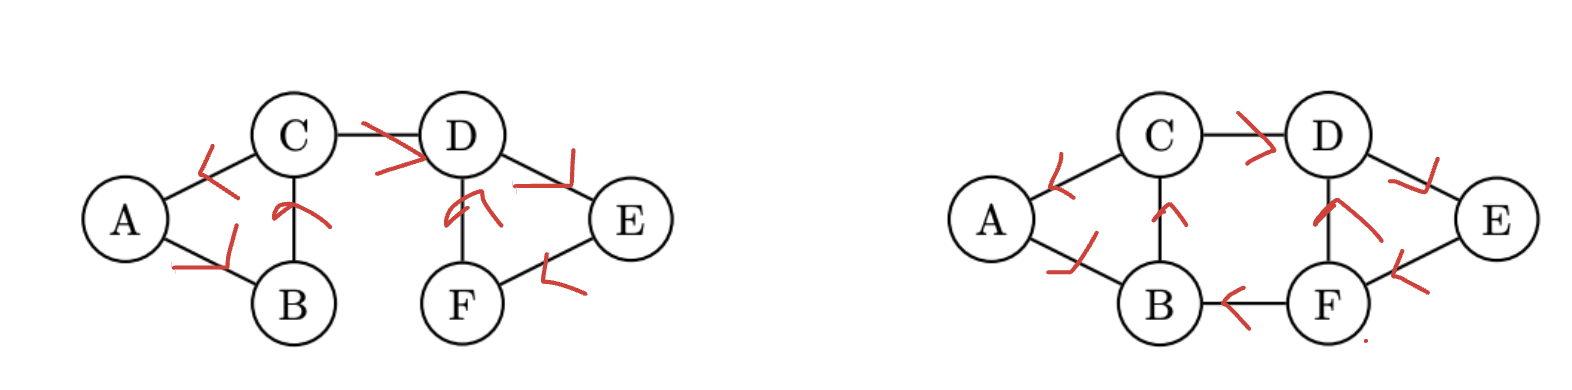
\includegraphics[width=1\linewidth]{cs3511/3_4.png}
        \end{center}

      \item Conjecture: the directed graph $G'$ formed by a DFS
        traversal on $G,$ taking edge $(u, v)$ if $v$ is visited by
        $u$ has a single connected component if and only if it is $2$-connected.

      \item Let us prove both sides of this conjecture. First, we
        prove that if we have a $2$-connected graph $G$, $G'$ is a
        single connected component.

        Assume some undirected graph $G$ is 2-connected, i.e., it
        remains connected if any edge $e \in E$ is removed. Then,
        consider a DFS starting at any vertex $r \in V.$ Assume for
        the sake of contradiction that the directed graph $G'$
        produced by this traversal has multiple connected components.
        Now consider the condensation graph of $G'.$

        For the sake of contradiction again, assume we have SCCs $U,
        V$ such that there is an edge $(u, v) \in E(G'),$ with $u \in
        U$ and $v \in V,$ and there is another path $p$ from $u$ to
        $v.$ Note that by definition, $p$ will have some edge $(u',
        n)$ where $n \not \in U,$ i.e., $n$ is in some other SCC $N$.
        There are two cases in the DFS of $G$ starting at $r$:
        \begin{itemize}
          \item If $(u, v)$ is traversed before $(u', n),$ then since
            $V$ is after $U$ in the topological order of the
            condensation graph of $G',$ all vertices $v \in V$ will
            occur in the postorder of $G$ before $u.$ Let the SCCs
            visited by path $p$ be represented as
            $$
            U \to P_1 \to P_2\to \ldots  \to P_r \to   V,
            $$
            and the first vertex visited by $p$ in SCC $S$ be
            $S^\star.$ In the postorder, $v^\star$ will be visited
            first before $u'$ since $p$ was not taken before $(u,
            v).$ Then, for the edge into $v^\star$ in $p$ to not be
            reversed, $v^\star$ must have been reached before $u.$
            However, this means all vertices in $V$ will be visited
            before $u, $ meaning we will take edge $(v, u)$ in $G',$
            contradicting the fact that $(u, v) \in E(G').$

          \item Otherwise, if $(u', n)$ is traversed before $(u, v),$
            all vertices in the subtree rooted at $N$ of the
            condensation graph of $G'$ will occur in the postorder
            before $u.$ This includes $v,$ but $v$ will take edge
            $(v, u)$ since $\{u, v\}$ is untraversed, producing $(v,
            u)$ in $G',$ which is a contradiction.
        \end{itemize}

        In either case, we derive a contradiction, meaning no other
        such path $p$ can exist in $G.$ Hence, removing $\{u, v\}$ in
        $G$ will mean there is no other such path from $u$ to $v,$
        and hence $G \setminus \{u, v\}$ is not connected. This is a
        contradiction of $G$'s $2$-connectedness, meaning $G'$ must
        be a single connected component.

        Now, let us prove that if $G'$ is a single connected
        component, $G$ is $2$-connected. Consider removing an
        arbitrary edge $\{u, v\} \in E(G).$ WLOG, this will
        correspond to removing some directed edge $(u, v) \in E(G').$
        Since $G'$ is a single strongly connected component, there is
        a path from $u$ to $v$ and a path from $v$ to $u.$ Removing
        $(u, v)$ means there still must exist a path from $v$ to $u,$
        since by definition $(u, v)$ was not included in this path.
        Hence, in the original undirected there still exists a path
        from $v$ to $u,$ and since this graph is a bidirectional, a
        path from $u$ to $v$ also exists.

        Let $G_d$ be the undirected graph produced by the deletion of
        $\{u, v\}$ in $G.$ By definition, every pair of vertices $a,
        b$ have some path $a \to b.$ Now consider $G_d,$ and for
        every pair of vertices $a, b$, construct the path by
        replacing every occurrence $(u, v)$ or $(v, u)$ with the
        undirected path from $v$ to $u$ (or flipped as required).
        Since such a $u \to v$ path always exist, we can always form
        a path from $a$ to $b$ for an arbitrary selection of $a, b$
        meaning $G_d$ is still connected. Hence, $G$ is $2$-connected.

      \item We use the above result to first produce $G'$ from $G,$
        and then determine if it is a single connected component.

        \begin{algorithm}
          \caption{Is $G$ $2$-connected?}
          \begin{algorithmic}
            \Procedure{TwoConnected}{$G$}
            \State $r = E(G)[0]$  \Comment{Arbitrary DFS root $r$.}
            \State $G' = \text{DFSAndTrackEdges}(G, r)$
            \Comment{$\mathcal O(|V| + |E|)$ DFS while tracking which
            directed edges taken.}

            \vspace{3mm}
            \State $\text{visited} \gets\text{DFS}(G', r)$
            \If{$\exists v \in V(G'),\ v \not \in \text{visited}$}
            \Comment{$\mathcal O(|V|)$}
            \State\Return{false}
            \EndIf

            $G' \gets \text{reversed}(G')$ \Comment{Flip direction of
            all edges in $\mathcal O(|V| + |E|)$.}

            \vspace{3mm}
            \State $\text{visited} \gets\text{DFS}(G', r)$
            \If{$\exists v \in V(G'),\ v \not \in \text{visited}$}
            \Comment{$\mathcal O(|V|)$}
            \State\Return{false}
            \EndIf

            \vspace{3mm}

            \State \Return{true} \Comment{$G'$ is a single connected
            component $\Leftrightarrow G$ is $2$-connected.}
            \EndProcedure
          \end{algorithmic}
        \end{algorithm}
    \end{enumerate}
\end{enumerate}
\end{document}
